\documentclass{article}
% Les différentes tailles :
% \tiny
% \scriptsize
% \footnotesize
% \small
% \normalsize
% \large
% \Large
% \LARGE
% \huge
% \Huge




\usepackage{tikz}
\usepackage{amsmath}
\usetikzlibrary{automata,arrows,backgrounds,calc,er,fit,intersections,matrix,patterns,positioning,snakes,shapes,through,trees}


\begin{document}


\pgfdeclarepatternformonly[/tikz/radius,\thickness,\size]{rings}
{\pgfpoint{-0.5*\size}{-0.5*\size}}
{\pgfpoint{0.5*\size}{0.5*\size}}
{\pgfpoint{\size}{\size}}
{
\pgfsetlinewidth{\thickness}
\pgfpathcircle\pgfpointorigin{\pgfkeysvalueof{/tikz/radius}}
\pgfusepath{stroke}
}
\newdimen\thickness
\tikzset{
radius/.initial=4pt,
size/.store in=\size, size=20pt,
thickness/.code={\thickness=#1},
thickness=0.75pt
}
% \begin{tikzpicture}[rings/.style={pattern=rings}]
% \filldraw [rings, radius=2pt, size=6pt] (0,0) rectangle +(1.5,2);
% \filldraw [rings, radius=2pt, size=8pt] (2,0) rectangle +(1.5,2);
% \filldraw [rings, radius=6pt, thickness=2pt] (0,2.5) rectangle +(1.5,2);
% \filldraw [rings, radius=8pt, thickness=4pt] (2,2.5) rectangle +(1.5,2);
% 
% \filldraw [rings, radius=8pt, thickness=4pt] (5,5) rectangle +(2.0,2.0);
% 
% \end{tikzpicture}
% 
% 
% \begin{tikzpicture}
% \foreach \y in {0,1,...,5} {
% \pgfmathparse{10-\y}\let\z\pgfmathresult
% \foreach \x in {\z,...,\y} {
% \draw (\x,\y)--(-\y,\x);
% }}
% \end{tikzpicture}
% 
% 
% 
% 
% 
% 
% \begin{tikzpicture}[scale=0.5]
% \foreach \y in {0,1,...,10} {
% \foreach \x in {0,1,...,10} {
% \fill[color=red!20] (\x,\y) circle (5pt);
% }}
% \end{tikzpicture}
% 
% \begin{tikzpicture}[scale=0.1]
% \foreach \y in {0,1,...,50} {
% \foreach \x in {0,1,...,50} {
% \fill[color=red!20] (\x,\y) circle (15pt);
% }}
% \end{tikzpicture}
% 
% 
% \begin{tikzpicture}[scale=0.1]
% \foreach \x in {0,1,...,50} {
% \fill[color=red!20] (\x,50-\x) circle (15pt);
% }
% \foreach \x in {1,2,...,50} {
% \fill[color=red!20] (\x-1,50-\x) circle (15pt);
% }
% \foreach \x in {0,1,...,49} {
% \fill[color=red!20] (\x+1,50-\x) circle (15pt);
% }
% \end{tikzpicture}
% 
% 
% 
% \begin{tikzpicture}[scale=0.5]
% \foreach \x in {0,1,...,10} {
% \fill[color=red!20] (\x,10-\x) circle (5pt);
% }
% \foreach \x in {1,2,...,10} {
% \fill[color=red!20] (\x-1,10-\x) circle (5pt);
% }
% \foreach \x in {0,1,...,9} {
% \fill[color=red!20] (\x+1,10-\x) circle (5pt);
% }
% \end{tikzpicture}
% 
% 




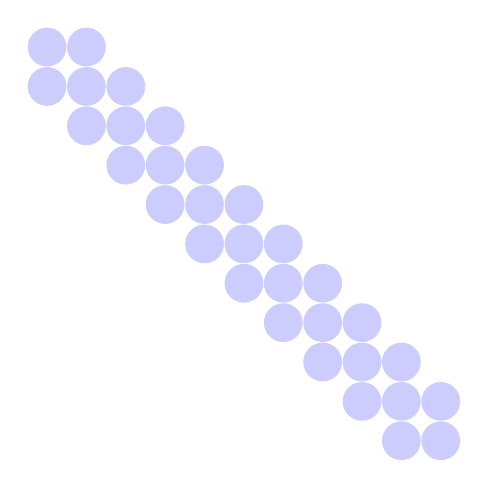
\begin{tikzpicture}[scale=0.5]
\foreach \x in {0,1,...,10} {
\fill[color=blue!20] (\x,10-\x) circle (14pt);
}
\foreach \x in {1,2,...,10} {
\fill[color=blue!20] (\x-1,10-\x) circle (14pt);
}
\foreach \x in {0,1,...,9} {
\fill[color=blue!20] (\x+1,10-\x) circle (14pt);
}
\end{tikzpicture}








% \begin{tikzpicture}
% [every left delimiter/.style={xshift=1ex},
% every right delimiter/.style={xshift=-1ex}]
% \matrix [matrix of math nodes,left delimiter=(,right delimiter=\}]
% {
% a_18 & a_1 & a_6 \\
% a_3 & a_5 & a_7 \\
% a_4 & a_9 & a_2 \\
% };
% \end{tikzpicture}


% 
% \begin{tikzpicture}[domain=0:8]
% %\draw[very thin,color=gray] (-0.1,-1.1) grid (8.2,3.9);
% \draw[->] (-0.2,4.0) -- (8.2,4.0) node[right] {$x$};
% \draw[->] (0,4.2) -- (0,-1.2) node[below] {$y$};
% \draw[->] (0,4.1) circle (0.1);
% \draw[red] plot[mark=x,mark repeat=2,smooth] file {matable1.table};
% \draw[blue] plot[mark=x,mark repeat=2,smooth] file {matable2.table};
% \draw plot[mark=x,mark repeat=2,smooth] file {matable3.table};
% 
% \draw[->,thick] (7,3) -- (7,1) node[right] {$g$};
% 
% 
% 
% \end{tikzpicture}






% 
% \begin{tikzpicture}
% [>=stealth',auto,text depth=1pt,
% every attribute/.style={fill=green!20,draw=black,thick},
% every entity/.style={inner sep=0pt,fill=blue!40,draw=black,thick},
% every relationship/.style={inner sep=8pt,rectangle,fill=red!15,draw=black,thick},
% pre/.style={<-,shorten <=1pt,>=stealth’,semithick}
% ]
% 
% \node[entity,fill opacity=0.0,draw opacity=0.0] (deb) at (7.5,0)  {$deb$};
% \node[entity,fill opacity=0.0,draw opacity=0.0] (fin) at (7.5,8)  {$fin$};
% 
% \node[entity] (x1) at (0,0) [label=left:$y_1$] {$x_1$};
% \node[entity] (x2) at (4,0) [label=right:$y_2$] {$x_2$};
% \node[attribute] (cosp) at (3,2) [label=right:$y_3$] {$cos(P)$};
% \node[attribute] (pq) at (2,4) [label=left:$y_4$] {$P-Q$};
% \node[attribute] (p2) at (2,6) [label=left:$y_5$] {$P^2$};
% \node[relationship] (fonction) at (2,8) {$f(x_1,x_2)= (x_1-cos(x_2))^2$};
% 
% 
% \path[->,thick,blue] (x1) edge node {$\bar{y_1}=\bar{y_4} \frac{\partial y_4}{\partial y_1}=\bar{y_4} $} (pq);
% \path[->,thick,blue] (x2) edge node [swap] {$\bar{y_2}=\bar{y_3} \frac{\partial y_3}{\partial y_2}=-\bar{y_3}sin(y_2)$} (cosp);
% \path[->,thick,blue] (cosp) edge node [swap] {$\bar{y_3}= \bar{y_4} \frac{\partial y_4}{\partial y_3}=-\bar{y_4}$} (pq);
% \path[->,thick,blue] (pq) edge node [swap] {$\bar{y_4}= \bar{y_5} \frac{\partial y_5}{\partial y_4}= 2\bar{y_5}y_4$} (p2);
% \path[->,thick,blue] (p2) edge node [swap] {$\bar{f}=\bar{y_5}=1$} (fonction);
% 
% 
% \path[->,ultra thick,red] (fin) edge node {Mode inverse} (deb);
% 
% \end{tikzpicture}
% 
% 
% 
% \begin{tikzpicture}
% [>=stealth',auto,text depth=1pt,
% every attribute/.style={fill=green!20,draw=black,thick},
% every entity/.style={inner sep=0pt,fill=blue!40,draw=black,thick},
% every relationship/.style={inner sep=8pt,rectangle,fill=red!15,draw=black,thick},
% pre/.style={<-,shorten <=1pt,>=stealth’,semithick}
% ]
% 
% \node[entity] (x1) at (0,0) [label=left:$y_1$ ] [label=right:$x_1$ ] {$x_1$};
% \node[entity] (x2) at (4,0) [label=left:$y_2$ ] [label=right:$x_2$] {$x_2$};
% \node[attribute] (cosp) at (3,2) [label=left:$y_3$] [label=right:$cos(y_2)$] {$cos(P)$};
% \node[attribute] (pq) at (2,4) [label=left:$y_4$]  [label=right:$y_1-cos(y_3)$] {$P-Q$};
% \node[attribute] (p2) at (2,6) [label=left:$y_5$]  [label=right:$y_4^2$] {$P^2$};
% \node[relationship] (fonction) at (2,8) [label=left:$y_6$] {$f(x_1,x_2)= (x_1-cos(x_2))^2$};
% 
% 
% 
% 
% \path[->,thick,blue] (x1) edge node {} (pq);
% \path[->,thick,blue] (x2) edge node [swap] {} (cosp);
% \path[->,thick,blue] (cosp) edge node [swap] {} (pq);
% \path[->,thick,blue] (pq) edge node [swap] {} (p2);
% \path[->,thick,blue] (p2) edge node [swap] {} (fonction);
% \end{tikzpicture}
% 
% 
% % \node[entity] (x1) at (0,0) [label=left:$y_1=x_1$] {$x_1$};
% % \node[entity] (x2) at (4,0) [label=right:$y_2x_2$] {$x_2$};
% % \node[attribute] (cosp) at (3,2) [label=right:$y_3=cos(y_2)$] {$cos(P)$};
% % \node[attribute] (pq) at (2,4) [label=left:$y_4=y_1-cos(y_3)$] {$P-Q$};
% % \node[attribute] (p2) at (2,6) [label=left:$y_5=y_4^2$] {$P^2$};
% % \node[relationship] (fonction) at (2,8) [label=left:$y_6$] {$f(x_1,x_2)= (x_1-cos(x_2))^2$};
% 
% 
% 
% 
% 
% 
% 
% \begin{tikzpicture}
% [>=stealth',auto,text depth=1pt,
% every attribute/.style={fill=green!20,draw=black,thick},
% every entity/.style={inner sep=0pt,fill=blue!40,draw=black,thick},
% every relationship/.style={inner sep=8pt,rectangle,fill=red!15,draw=black,thick},
% pre/.style={<-,shorten <=1pt,>=stealth’,semithick}
% ]
% \node[entity] (x1) at (0,0) [label=left:$y_1$] {$x_1$};
% \node[entity] (x2) at (4,0) [label=right:$y_2$] {$x_2$};
% \node[attribute] (cosp) at (3,2) [label=right:$y_3$] {$cos(P)$};
% \node[attribute] (pq) at (2,4) [label=left:$y_4$] {$P-Q$};
% \node[attribute] (p2) at (2,6) [label=left:$y_5$] {$P^2$};
% \node[relationship] (fonction) at (2,8) [label=left:$y_6$] {$f(x_1,x_2)= (x_1-cos(x_2))^2$};
% 
% 
% \path[->,thick,blue] (x1) edge node {} (pq);
% \path[->,thick,blue] (x2) edge node [swap] {} (cosp);
% \path[->,thick,blue] (cosp) edge node [swap] {} (pq);
% \path[->,thick,blue] (pq) edge node [swap] {} (p2);
% \path[->,thick,blue] (p2) edge node [swap] {} (fonction);
% \end{tikzpicture}
% 
% 
% 
% 
% 
% 
% 
% 
% 
% \def\xmin{-1}
% \def\xmax{4}
% \def\xk1{1.2894652}
% 
% 
% \begin{tikzpicture}[samples=100,domain=\xmin:\xmax]
% \draw[very thin,color=gray] (-4.2,-0.5) grid (1.2,5);
% \draw[->] ({\xmin-0.1},0) -- ({\xmax+0.1},0) node[right] {$x$};
% \draw[->] (0,-1) -- (0,5) node[above] {$f(x)$};
% \draw[color=blue] plot ((\x,{-3*sin(\x r)+4*\x)/6}) node[right] {$f(x)$};
% \draw[-] (3.5,0) node[below] {$x_k$} -- (3.5,{(-3*sin(3.5 r)+4*(3.5))/6});
% \begin{scope}
% \clip (-3.5,0) rectangle (0,5);
% \draw[color=red] plot ((\x,{(3*sin(-3.5 r)+4*(3.5) + (3*cos(-3.5 r)-4)*(\x+3.5))/6});
% \end{scope}
% \node [below] at (\xk1,0)  {$x_{k+1}$}; 
% 
% 
% 
% \draw[-] (\xk1,0) -- (\xk1,{(-3*sin(\xk1 r)+4*(\xk1))/6}) ;
% \begin{scope}
% \clip (\xk1,0) rectangle (0,5);
% \draw[color=red] plot ((\x,{(3*sin(\xk1 r)-4*(\xk1) + (3*cos(\xk1 r)-4)*(\x-\xk1))/6});
% \end{scope}
% 
% \node [below] at (-.5,0)  {$x_{k+2}$}; 
% \node  at (-2,3.5)  {$x_{k+1}\leftarrow x_k-\frac{f(x)}{f'(x)}$}; 
% \end{tikzpicture}
% 
% 
% 
% 
% 
% 
% 
% 
% 
% 
% 
% 
% 
% 
% 
% 
% 
% 
% 
% 
% 
% 
% 
% 
% 
% 
% 
% 
% 
% 
% 
% \def\xmin{-4}
% \def\xmax{1}
% \def\xk1{-1.2894652}
% 
% 
% \begin{tikzpicture}[samples=100,domain=\xmin:\xmax]
% \draw[very thin,color=gray] (-4.2,-0.5) grid (1.2,5);
% \draw[->] ({\xmin-0.1},0) -- ({\xmax+0.1},0) node[right] {$x$};
% \draw[->] (0,-1) -- (0,5) node[above] {$f(x)$};
% \draw[color=blue] plot ((\x,{3*sin(\x r)-4*\x)/6}) node[right] {$f(x)$};
% \draw[-] (-3.5,0) node[below] {$x_k$} -- (-3.5,{(3*sin(-3.5 r)+4*(3.5))/6});
% \begin{scope}
% \clip (-3.5,0) rectangle (0,5);
% \draw[color=red] plot ((\x,{(3*sin(-3.5 r)+4*(3.5) + (3*cos(-3.5 r)-4)*(\x+3.5))/6});
% \end{scope}
% \node [below] at (\xk1,0)  {$x_{k+1}$}; 
% 
% 
% 
% \draw[-] (\xk1,0) -- (\xk1,{(3*sin(\xk1 r)-4*(\xk1))/6}) ;
% \begin{scope}
% \clip (\xk1,0) rectangle (0,5);
% \draw[color=red] plot ((\x,{(3*sin(\xk1 r)-4*(\xk1) + (3*cos(\xk1 r)-4)*(\x-\xk1))/6});
% \end{scope}
% 
% \node [below] at (-.5,0)  {$x_{k+2}$}; 
% \node  at (-2,3.5)  {$x_{k+1}\leftarrow x_k-\frac{f(x)}{f'(x)}$}; 
% \end{tikzpicture}
% 
% 
% 
% 
% 
% \begin{tikzpicture}[domain=0:4]
% \draw[very thin,color=gray] (-0.1,-1.1) grid (3.9,3.9);
% \draw[->] (-0.2,0) -- (4.2,0) node[right] {$x$};
% \draw[->] (0,-1.2) -- (0,4.2) node[above] {$f(x)$};
% \draw[color=red] plot (\x,\x) node[right] {$f(x) =x$};
% \draw[color=blue] plot (\x,{sin(\x r)}) node[right] {$f(x) = \sin x$};
% \draw[color=orange] plot (\x,{0.05*exp(\x)}) node[right] {$f(x) = \frac{1}{20} \mathrm e^x$};
% \end{tikzpicture}
% 
% 
% 
% 
% 
% 
% \begin{tikzpicture}
% [pointnoir/.style={circle,draw=black,fill=black,thin,
% inner sep=0pt,minimum size=6pt},
% pointblanc/.style={circle,draw=black,fill=white,thin,
% inner sep=0pt,minimum size=6pt},
% petitpoint/.style={circle,draw=black,fill=black,thin,
% inner sep=0pt,minimum size=2pt}, %Minimum size parce que si on écrit qqch ça l'entoure donc plus que le min
% fleche/.style={<-,>=stealth,thick},
% flecheinv/.style={->,>=stealth, line width=2pt},
% rien/.style={circle,draw=black,fill=black,thin,inner sep=0pt,minimum size=0pt}
% ]
% 
% 
% % \node (point1) at (3.5,0.3) [petitpoint] {};
% % \node (point2) at (4.0,0.3) [petitpoint] {};
% % \node (point3) at (4.5,0.3) [petitpoint] {};
% 
% \node at ( 0,0) [pointnoir] (a) {};
% \node at ( 6,0) [pointnoir] (g) {}
% edge [fleche] (a);
% \node at ( 7,0) [pointnoir] (h) {}
% edge [fleche] (g);
% \node at ( 8,0) [pointnoir] (i) {}
% edge [fleche] (h);
% \node at ( 9,0) [pointnoir] (j) {}
% edge [fleche] (i);
% \node at ( 10,0) [rien] (k) {}
% edge [fleche] (j);
% 
% 
% \node at ( 6,-0.5) [rien] (r) {};
% \node at ( 7,-0.5) [pointblanc] (s) {}
% edge [flecheinv] (r);
% \node at ( 8,-0.5) [pointblanc] (t) {}
% edge [flecheinv] (s);
% \node at ( 9,-0.5) [pointblanc] (u) {}
% edge [flecheinv] (t);
% \node at ( 10,-0.5) [pointblanc] (v) {}
% edge [flecheinv] (u);
% \node at ( 11,-0.5) [rien] (w) {}
% edge [flecheinv] (v);
% 
% 
% 
% \node at ( 0,-1) [pointnoir] (a) {};
% \node at ( 1,-1) [pointnoir] (f) {}
% edge [fleche] (a);
% \node at ( 2,-1) [pointnoir] (g) {}
% edge [fleche] (f);
% \node at ( 3,-1) [pointnoir] (h) {}
% edge [fleche] (g);
% \node at ( 4,-1) [pointnoir] (i) {}
% edge [fleche] (h);
% \node at ( 5,-1) [rien] (j) {}
% edge [fleche] (i);
% 
% 
% 
% \node at ( 0,-1.5) [rien] (r) {};
% \node at ( 1,-1.5) [pointblanc] (s) {}
% edge [flecheinv] (r);
% \node at ( 2,-1.5) [pointblanc] (t) {}
% edge [flecheinv] (s);
% \node at ( 3,-1.5) [pointblanc] (u) {}
% edge [flecheinv] (t);
% \node at ( 4,-1.5) [pointblanc] (v) {}
% edge [flecheinv] (u);
% \node at ( 5,-1.5) [pointblanc] (w) {}
% edge [flecheinv] (v);
% \node at ( 6,-1.5) [rien] (x) {}
% edge [flecheinv] (w);
% 
% 
% 
% 
% \draw[->,>=stealth,line width=2pt] (-0.5,0) -- (-0.5,-1.5);
% \node (temps) at (-1.1,-0.75) {temps};
% 
% 
% 
% 
% \end{tikzpicture}
% 
% 
% 
% 
% 
% 
% 
% 
% 
% 
% 
% 
% 
% 
% 
% 
% 
% 
% 
% 
% 
% \begin{tikzpicture}
% [pointnoir/.style={circle,draw=black,fill=black,thin,
% inner sep=0pt,minimum size=8pt},
% pointblanc/.style={circle,draw=black,fill=white,thin,
% inner sep=0pt,minimum size=8pt},
% petitpoint/.style={circle,draw=black,fill=black,thin,
% inner sep=0pt,minimum size=2pt}, %Minimum size parce que si on écrit qqch ça l'entoure donc plus que le min
% fleche/.style={<-,>=stealth,thick},
% flecheinv/.style={->,>=stealth, line width=2pt},
% rien/.style={circle,draw=black,fill=black,thin,inner sep=0pt,minimum size=0pt}
% ]
% 
% \draw[decorate,decoration=brace,very thick](0,0.5) -- (5,0.5);
% \node (P) at (2.5,0.8) { $p$};
% 
% \node at ( 0,0) [pointnoir] (a) {};
% \node at ( 5,0) [pointnoir] (b) {}
% edge [fleche] (a);
% \node at ( 10,0) [rien] (c) {}
% edge [fleche] (b);
% \node at (10 ,-0.2) [rien] (c) {};
% \node at (11,-0.2) [rien] (d) {}
% edge [flecheinv] (c);
% \node at ( 5,-0.5) [pointblanc] (e) {};
% \node at ( 9,-0.5) [rien] (f) {}
% edge [fleche] (e);
% \node at (9 ,-0.7) [rien] (g) {};
% \node at (10,-0.7) [rien] (h) {}
% edge [flecheinv] (g);
% 
% \node (point1) at (6,-1) [petitpoint] {};
% \node (point2) at (6.5,-1) [petitpoint] {};
% \node (point3) at (7,-1) [petitpoint] {};
% 
% 
% \node at (5,-1.5) [pointblanc] (i) {};
% \node at (5,-1.7) [rien] (j) {};
% \node at (6,-1.7) [rien] (k) {}
% edge [flecheinv] (j);
% 
% 
% 
% \node at ( 0,-2) [pointblanc] (k) {};
% \node at ( 4,-2) [rien] (l) {}
% edge [fleche] (k);
% \node at (4,-2.2) [rien] (m) {};
% \node at (5,-2.2) [rien] (n) {}
% edge [flecheinv] (m);
% 
% \node (point1) at (1,-2.4) [petitpoint] {};
% \node (point2) at (1.5,-2.4) [petitpoint] {};
% \node (point3) at (2,-2.4) [petitpoint] {};
% 
% \node at ( 0,-3) [pointblanc] (i) {};
% \node at ( 1,-3) [rien] (j) {}
% edge [fleche] (i);
% \node at (1 ,-3.2) [rien] (k) {};
% \node at (2,-3.2) [rien] (l) {}
% edge [flecheinv] (k);
% \node at ( 0,-3.5) [pointblanc] (m) {};
% \node at (0 ,-3.7) [rien] (n) {};
% \node at (1,-3.7) [rien] (o) {}
% edge [flecheinv] (n);
% \draw[->,>=stealth,line width=2pt] (-0.5,0) -- (-0.5,-3.7);
% \node (temps) at (-1.1,-1.8) {temps};
% \end{tikzpicture}
% 
% \vspace{1cm}
% 
% 
% 
% 
% 
% 
% 
% 
% \begin{tikzpicture}
% [pointnoir/.style={circle,draw=black,fill=black,thin,
% inner sep=0pt,minimum size=8pt},
% pointblanc/.style={circle,draw=black,fill=white,thin,
% inner sep=0pt,minimum size=8pt},
% petitpoint/.style={circle,draw=black,fill=black,thin,
% inner sep=0pt,minimum size=2pt}, %Minimum size parce que si on écrit qqch ça l'entoure donc plus que le min
% fleche/.style={<-,>=stealth,thick},
% flecheinv/.style={->,>=stealth, line width=2pt},
% rien/.style={circle,draw=black,fill=black,thin,inner sep=0pt,minimum size=0pt}
% ]
% \node at ( 0,0) [pointnoir] (a) {};
% \node at ( 10,0) [rien] (b) {}
% edge [fleche] (a);
% \node (I1) at (0.5,0.4) { $I_1$};
% \node (I2) at (1.5,0.4) { $I_2$};
% \node (I3) at (2.5,0.4) { $I_3$};
% \node (point1) at (3.5,0.4) [petitpoint] {};
% \node (point2) at (4.0,0.4) [petitpoint] {};
% \node (point3) at (4.5,0.4) [petitpoint] {};
% \node (Ip2) at (8.5,0.4) { $I_{p-2}$};
% \node (Ip1) at (9.5,0.4) { $I_{p-1}$};
% \node at (10 ,-0.2) [rien] (c) {};
% \node at (11,-0.2) [rien] (d) {}
% edge [flecheinv] (c);
% \node (Ip) at (10.5,-0.6) {$\overline{I_{p}}$};
% \node at ( 0,-1) [pointblanc] (e) {};
% \node at ( 9,-1) [rien] (f) {}
% edge [fleche] (e);
% \node at (9 ,-1.2) [rien] (g) {};
% \node at (10,-1.2) [rien] (h) {}
% edge [flecheinv] (g);
% \node (Ip3) at (9.5,-1.6) {$\overline{I_{p-1}}$};
% \node at ( 0,-3) [pointblanc] (i) {};
% \node at ( 1,-3) [rien] (j) {}
% edge [fleche] (i);
% \node (I1) at (0.5,-2.6) { $I_1$};
% \node at (1 ,-3.2) [rien] (k) {};
% \node at (2,-3.2) [rien] (l) {}
% edge [flecheinv] (k);
% \node (Ip4) at (1.5,-3.6) {$\overline{I_{2}}$};
% \node at ( 0,-4) [pointblanc] (m) {};
% \node at (0 ,-4.2) [rien] (n) {};
% \node at (1,-4.2) [rien] (o) {}
% edge [flecheinv] (n);
% \node (Ip5) at (0.5,-4.6) {$\overline{I_{1}}$};
% \draw[->,>=stealth,line width=2pt] (-0.5,0) -- (-0.5,-4.2);
% \node (temps) at (-1.1,-2.1) {temps};
% \end{tikzpicture}
% 
% \vspace{1cm}
% 
% 
% 
% \begin{tikzpicture}
% [pointnoir/.style={circle,draw=black,fill=black,thin,
% inner sep=0pt,minimum size=6pt},
% pointblanc/.style={circle,draw=black,fill=white,thin,
% inner sep=0pt,minimum size=6pt},
% petitpoint/.style={circle,draw=black,fill=black,thin,
% inner sep=0pt,minimum size=2pt}, %Minimum size parce que si on écrit qqch ça l'entoure donc plus que le min
% fleche/.style={<-,>=stealth,thick},
% flecheinv/.style={->,>=stealth, line width=2pt},
% rien/.style={circle,draw=black,fill=black,thin,inner sep=0pt,minimum size=0pt}
% ]
% 
% \node (I1) at (0.5,0.3) { $I_1$};
% \node (I2) at (1.5,0.3) { $I_2$};
% \node (I3) at (2.5,0.3) { $I_3$};
% \node (point1) at (3.5,0.3) [petitpoint] {};
% \node (point2) at (4.0,0.3) [petitpoint] {};
% \node (point3) at (4.5,0.3) [petitpoint] {};
% 
% \node (Ip1) at (8.5,0.3) { $I_{p-2}$};
% \node (Ip2) at (9.5,0.3) { $I_{p-1}$};
% 
% 
% 
% \node at ( 0,0) [pointnoir] (a) {};
% \node at ( 1,0) [pointnoir] (b) {}
% edge [fleche] (a);
% \node at ( 2,0) [pointnoir] (c) {}
% edge [fleche] (b);
% \node at ( 3,0) [pointnoir] (d) {}
% edge [fleche] (c);
% \node at ( 4,0) [pointnoir] (e) {}
% edge [fleche] (d);
% \node at ( 5,0) [pointnoir] (f) {}
% edge [fleche] (e);
% \node at ( 6,0) [pointnoir] (g) {}
% edge [fleche] (f);
% \node at ( 7,0) [pointnoir] (h) {}
% edge [fleche] (g);
% \node at ( 8,0) [pointnoir] (i) {}
% edge [fleche] (h);
% \node at ( 9,0) [pointnoir] (j) {}
% edge [fleche] (i);
% \node at ( 10,0) [rien] (k) {}
% edge [fleche] (j);
% 
% 
% 
% 
% \node (I1) at (0.5,-0.7) { $\overline{I_1}$};
% \node (I2) at (1.5,-0.7) { $\overline{I_2}$};
% \node (I3) at (2.5,-0.7) { $\overline{I_3}$};
% 
% 
% \node (Ip3) at (8.5,-0.7) { $\overline{I_{p-2}}$};
% \node (Ip4) at (9.5,-0.7) { $\overline{I_{p-1}}$};
% \node (Ip5) at (10.5,-0.7) {$\overline{I_{p}}$};
% 
% \node at ( 0,-1) [rien] (l) {};
% \node at ( 1,-1) [pointblanc] (m) {}
% edge [flecheinv] (l);
% \node at ( 2,-1) [pointblanc] (n) {}
% edge [flecheinv] (m);
% \node at ( 3,-1) [pointblanc] (o) {}
% edge [flecheinv] (n);
% \node at ( 4,-1) [pointblanc] (p) {}
% edge [flecheinv] (o);
% \node at ( 5,-1) [pointblanc] (q) {}
% edge [flecheinv] (p);
% \node at ( 6,-1) [pointblanc] (r) {}
% edge [flecheinv] (q);
% \node at ( 7,-1) [pointblanc] (s) {}
% edge [flecheinv] (r);
% \node at ( 8,-1) [pointblanc] (t) {}
% edge [flecheinv] (s);
% \node at ( 9,-1) [pointblanc] (u) {}
% edge [flecheinv] (t);
% \node at ( 10,-1) [pointblanc] (v) {}
% edge [flecheinv] (u);
% \node at ( 11,-1) [rien] (w) {}
% edge [flecheinv] (v);
% 
% \draw[->,>=stealth,line width=2pt] (-0.5,0) -- (-0.5,-1);
% \node (temps) at (-1.1,-0.5) {temps};
% 
% 
% 
% 
% \end{tikzpicture}
% 
% 
% 
% 
% 
% 
% 
% 
% 
% 
% 
% 
% 
% 
% 
% 
% 
% 
% 
% 
% 
% 
% \begin{tikzpicture}
% [point/.style={circle,draw=black,fill=black,thin,
% inner sep=0pt,minimum size=4pt},
% fleche/.style={<-,shorten <=1pt,>=stealth',semithick}
% ]
% %shorten pour que la flèche s'arrete avant d'atteindre le point
% 
% \node at ( 0,0) [point] (a) {};
% \node at ( 10,0) [point] (b) {}
% edge [fleche] (a);
% \end{tikzpicture}
% 
% 
% 
% 
% 
% 
% 
% 
% 
% \begin{tikzpicture}
% [point/.style={circle,draw=black,fill=black,thin,
% inner sep=0pt,minimum size=4pt},
% transition/.style={rectangle,draw=black!50,fill=black!20,thick,
% inner sep=0pt,minimum size=4mm}]
% \node at ( 0,0) [point] (a) {};
% \node at ( 1,0) [point] (b) {}
% edge [<-] (a);
% \node at ( 2,0) [point] (c) {}
% edge [<-] (b);
% \node at ( 3,0) [point] (d) {}
% edge [<-] (c);
% \node at ( 4,0) [point] (e) {}
% edge [<-] (d);
% \node at ( 5,0) [point] (f) {}
% edge [<-] (d);
% \node at ( 6,0) [point] (g) {}
% edge [<-] (e);
% \end{tikzpicture}
% 
% 
% 
% 
% 
% 
% 
% \begin{tikzpicture}
% % \draw [help lines] (0,0) grid (3,2);
% \fill [black] (0,0) circle (2pt);
% \fill [black] (1,0) circle (2pt);
% \fill [black] (2,0) circle (2pt);
% \fill [black] (3,0) circle (2pt);
% \fill [black] (4,0) circle (2pt);
% \fill [black] (5,0) circle (2pt);
% \fill [black] (6,0) circle (2pt);
% \fill [black] (7,0) circle (2pt);
% \draw [->] (0,0)--(1,0);
% 
% 
% 
% 
% \end{tikzpicture}
% 
% \vspace{3cm}
% 
% \begin{tikzpicture}
% \draw [help lines] (0,0) grid (3,2);
% \fill [red] ($2*(1,1)$) circle (2pt);
% \fill [green] (${1+1}*(1,.5)$) circle (2pt);
% \fill [blue] ($cos(0)*sin(90)*(1,1)$) circle (2pt);
% \fill [black] (${3*(4-3)}*(1,0.5)$) circle (2pt);
% \end{tikzpicture}
% 
% 
% 
% \vspace{3cm}
% 
% 
% 
% 
% 
% 
% 
% \begin{tikzpicture}[scale=3]
% \clip (-0.1,-0.2) rectangle (1.1,1.51);
% \draw[step=.5cm,gray,very thin] (-1.4,-1.4) grid (1.4,1.4);
% \draw[->] (-1.5,0) -- (1.5,0);
% \draw[->] (0,-1.5) -- (0,1.5);
% \draw (0,0) circle (1cm);
% \filldraw[fill=green!20,draw=green!50!black] (0,0) -- (3mm,0mm) arc
% (0:30:3mm) -- cycle;
% \draw[red,very thick]
% (30:1cm) -- +(0,-0.5);
% \draw[blue,very thick]
% (30:1cm) ++(0,-0.5) -- (0,0);
% \path [name path=upward line] (1,0) -- (1,1);
% \path [name path=sloped line] (0,0) -- (30:1.5cm);
% \draw [name intersections={of=upward line and sloped line, by=x}]
% [very thick,orange] (1,0) -- (x);
% \end{tikzpicture}
% 
% \vspace{3cm}
% 
% 
% 
% 
% 
% 
% 
% \begin{tikzpicture}[scale=3]
% \clip (-0.1,-0.2) rectangle (1.1,1.51);
% \draw[step=.5cm,gray,very thin] (-1.4,-1.4) grid (1.4,1.4);
% \draw[->] (-1.5,0) -- (1.5,0);
% \draw[->] (0,-1.5) -- (0,1.5);
% \draw (0,0) circle (1cm);
% \filldraw[fill=green!20,draw=green!50!black] (0,0) -- (3mm,0mm) arc
% (0:30:3mm) -- cycle;
% \draw[red,very thick]
% (30:1cm) -- +(0,-0.5);
% \draw[blue,very thick]
% (30:1cm) ++(0,-0.5) -- (0,0);
% \path [name path=upward line] (1,0) -- (1,1);
% \path [name path=sloped line] (0,0) -- (30:1.5cm);
% \draw [name intersections={of=upward line and sloped line, by=x}]
% [very thick,orange] (1,0) -- (x);
% \end{tikzpicture}
% 
% \vspace{3cm}
% 
% 
% 
% 
% 
% 
% 
% 
% \begin{tikzpicture}[scale=3]
% \begin{scope}
% \draw[clip] (0,0) circle (1cm);
% \fill[green!15] (-80:1cm) rectangle (1,1);
% \end{scope}
% \draw[step=0.5cm,gray,very thin] (-1.0,-1.0) grid (1.0,1.0);
% \draw[dashed,red!50!black] (0,0) -- (80:1cm);
% \filldraw[fill=red!20,draw=red!50!black] (0,0) -- (1.4mm,0mm) arc
% (0:80:1.4mm) -- cycle;
% %(10:1cm) correspond à un angle de 30 degrés de longueur 1cm
% %(30:1cm |- 0,0) correspond à l'intersection de ma droite partant de 30:1cm
% % à la droite 0.0
% \draw[green, thick] (80:1cm) -- (-80:1cm);
% \draw[<->,brown,thick] (130:1cm) -- (0,0); 
% 
% \draw[->,thick] (0,0) -- (1.1,0);
% \node (rayon) at (-0.5,0.6) {{\scriptsize $\gamma_1 \lVert \nabla f(x) \rVert$}};
% \node (grad) at (1.1,-0.1) {{\scriptsize $-\nabla f(x)$}};
% 
% \draw[<->,thick] (0.0,-0.4) -- (80:1cm |- 0.0 ,-0.4);
% \node (largeur) at (0.1,-0.5) {{\scriptsize $\gamma_0 \lVert \nabla f(x) \rVert$}};
% \node (anglemax) at (0.2,0.1) {{\scriptsize $\theta_{max}$}};
% 
% \node (titre_zone1) at (1.2,1.2) {{\scriptsize Zone des directions}};
% \node (titre_zone2) at (1.2,1.1) {{\scriptsize suffisamment descendantes}};
% 
% \draw[<-,thick] (0.6,0.2) -- (titre_zone2);
% 
% \end{tikzpicture}
% \vspace{3cm}
% 
% \begin{tikzpicture}
% %définition des styles 
% [>=stealth',auto,text depth=1pt,
% every attribute/.style={fill=green!20,draw=black,thick},
% every entity/.style={inner sep=0pt,fill=blue!40,draw=black,thick},
% every relationship/.style={inner sep=8pt,rectangle,fill=red!15,draw=black,thick},
% pre/.style={<-,shorten <=1pt,>=stealth’,semithick}
% ]
% \node[entity,fill opacity=0.0,draw opacity=0.0] (deb) at (5.5,0)  {$deb$};
% \node[entity,fill opacity=0.0,draw opacity=0.0] (fin) at (5.5,8)  {$fin$};
% \node[entity] (x1) at (0,0) [label=left:$y_1$] {$x_1$};
% \node[entity] (x2) at (4,0) [label=right:$y_2$] {$x_2$};
% \node[attribute] (cosp) at (3,2) [label=right:$y_3$] {$cos(P)$};
% \node[attribute] (pq) at (2,4) [label=left:$y_4$] {$P-Q$};
% \node[attribute] (p2) at (2,6) [label=left:$y_5$] {$P^2$};
% \node[relationship] (fonction) at (2,8) [label=left:$y_6$] {$f(x_1,x_2)= (x_1-cos(x_2))^2$};
% 
% 
% \path[->,thick,blue] (x1) edge node {$\dot{y_1} $} (pq);
% \path[->,thick,blue] (x2) edge node [swap] {$\dot{y_2} $} (cosp);
% \path[->,thick,blue] (cosp) edge node [swap] {$\dot{y_3}=-\dot{y_2}sin(y_2)$} (pq);
% \path[->,thick,blue] (pq) edge node [swap] {$\dot{y_4}=\dot{y_1}-\dot{y_3}$} (p2);
% \path[->,thick,blue] (p2) edge node [swap] {$\dot{y_5}=2\dot{y_4}y_4$} (fonction);
% 
% 
% \path[->,ultra thick,red] (deb) edge node [swap] {Mode directe} (fin);
% 
% \end{tikzpicture}
% 
% \vspace{3cm}
% 







\end{document}
